\documentclass[10pt]{article}
\usepackage[polish]{babel}
\usepackage[utf8]{inputenc}
\usepackage[T1]{fontenc}
\usepackage{graphicx}
\usepackage[export]{adjustbox}
\graphicspath{ {./images/} }

\title{LIGA MATEMATYCZNA PAŹDZIERNIK 2011 SZKOŁA PODSTAWOWA }

\author{}
\date{}


\begin{document}
\maketitle
\section*{ZADANIE 1.}
Ile jest liczb dziesięciocyfrowych, które można napisać przy użyciu cyfr 1, 2, 3 (nie trzeba wykorzystać wszystkich cyfr jednocześnie) tak, aby każde dwie sąsiednie cyfry różniły się o jeden?

\section*{ZADANIE 2.}
W klasie jest 27 uczniów. Każdy z nich uprawia przynajmniej jedną z trzech dyscyplin sportowych: piłkę nożną, pływanie lub tenis. Najwięcej uczniów uprawia pływanie, a najmniej tenis. W piłkę nożną gra 15 uczniów. Tylko jeden uczeń uprawia jednocześnie trzy dyscypliny sportu. Dwoje uprawia tenis i piłkę nożną. Czworo uprawia pływanie i piłkę nożną, troje - tenis i pływanie. Ilu uczniów uprawia pływanie? Ilu uczniów uprawia tylko tenis?

\section*{ZADANIE 3.}
Rozłożono sto cukierków na pięciu talerzach:

\begin{itemize}
  \item na pierwszym i drugim talerzu znalazły się 52 cukierki;
  \item na drugim i trzecim talerzu 43 cukierki;
  \item na trzecim i czwartym - 34 cukierki;
  \item na czwartym i piątym - 30 cukierków.
\end{itemize}

Ile cukierków znajdowało się na każdym talerzu?

\section*{ZADANIE 4.}
W schronisku dla zwierząt była taka sama liczba psów i kotów. Trzecia część psów i połowa kotów znalazła opiekunów. Po sześć psów i jednego kota zgłoszą się właściciele i wtedy w schronisku będzie więcej kotów niż psów. Ile psów mogło znajdować się w schronisku na początku? Podaj wszystkie możliwości.

\section*{ZADANIE 5.}
Prostokąt podzielono na siedem kwadratów. Bok każdego z zaciemnionych kwadratów ma długość 8. Jaką długość ma bok największego kwadratu?\\
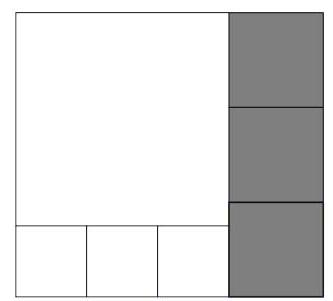
\includegraphics[max width=\textwidth, center]{2024_11_21_f039bcee261536a43d78g-1}


\end{document}